\documentclass[11pt]{article}

\usepackage[margin=1in]{geometry}
\usepackage{amsmath,amssymb}
\usepackage{booktabs}
\usepackage{graphicx}
\usepackage{hyperref}
\usepackage{microtype}

\newcommand{\UM}{U_{\mathrm{M}}}
\newcommand{\Usc}{U_{\mathrm{sc}}}
\newcommand{\Urel}{U_{\mathrm{rel}}}
\newcommand{\BSBM}{B_{\mathrm{S}}/B_{\mathrm{M}}}
\newcommand{\code}[1]{\texttt{#1}}

\title{Observation Models for Lunar Prospector Electron-Reflectometer\\
Loss-Cone Inference: A Controlled Three-Method Experiment}
\author{ESPG Lunar Potential Map Project}
\date{11 July 2026}

\begin{document}
\maketitle

\begin{abstract}
We compare three observation models for estimating lunar surface potential from
Lunar Prospector Electron Reflectometer (LP ER) loss-cone measurements.  The
experiment follows a telemetry audit showing that the existing calibrated-flux
Poisson implementation overstates the raw count scale by a median factor of
120.9 and ignores logarithmic counter intervals.  The candidates are (1) a
negative-binomial likelihood integrated over the raw Format-3 compression
interval, (2) a row-conditional Student-$t$ model for centered log flux, and (3)
the smooth pairwise Lillis objective with empirical uncertainty calibration.
The panel was frozen before candidate fitting: three benchmark spectra, seven
discovery spectra, and fifty temporally later confirmation spectra.  Smooth
Lillis alone reproduces the published primary benchmark, obtaining
$\Urel=-164.4$~V against the published $-171$~V, while interval counts and
conditional shape obtain $-244.2$ and $-225.2$~V.  All methods place the beam
amplitude at its upper bound.  Across confirmation spectra, boundary-hit rates
are 82\%, 64\%, and 56\%, respectively, and method differences frequently
exceed 100~V.  In matched simulations with nuisance physics fixed, all three
recover voltage accurately, with median absolute errors of 4--9~V.  The
contrast shows that count reconstruction was a major error but not the sole
cause of disagreement: the shared forward model is misspecified for substantial
real-data structure.  No candidate is advanced as a production likelihood.
\end{abstract}

\section{Scientific Background}

Electron reflectometry infers electrostatic potential from the angular deficit
of electrons that would otherwise mirror above the lunar surface.  For a
surface-connected magnetic field line, electrons within a loss cone are removed
or altered by interaction with the surface and electrostatic potential.  The
energy dependence of the loss-cone boundary contains information about lunar
surface potential, while the angular boundary also depends on the magnetic
field ratio.

The LP ER three-dimensional product contains 15 energy channels and 88 look
directions.  A distribution is acquired over approximately one half-spin and
sampled once per 16 spins.  The instrument does not transmit unbounded integer
counters.  It truncates each counter into an eight-bit logarithmic code.  Ground
processing decompresses that code, applies exposure, response, dead-time, and
geometric-factor corrections, and archives differential flux.  Approximately
10 counts~s$^{-1}$ of instrumental and cosmic-ray background are retained.

This distinction became central after a nominal Cash fit moved the published
benchmark from approximately $\Urel=-162$~V under smooth Lillis to
$-253$~V and returned a reduced deviance near 1421.  A raw telemetry audit found
that the production inverse
\begin{equation}
  C_{ej}^{\mathrm{prod}} = F_{ej} G E_e
  \frac{2.5~\mathrm{s}}{N_{\mathrm{az},j}}
\end{equation}
uses the half-spin support as though it were per-bin live time.  Accounting for
angular scanning and energy-sweep duty gives the idealized scale
\begin{equation}
  \Delta t_{ej} \simeq
  \frac{P_{\mathrm{spin}}}{256N_{\mathrm{az},j}},
\end{equation}
with further energy dependence in archive processing.  Direct Format-3
comparison gives a median production-to-raw-lower count ratio of 120.9.  This
explains most of the nominal information inflation, but a first-order rescaling
would still leave reduced deviance near 12 rather than one.

\section{Common Physical Model}

All three attempts use an identical forward model.  The loss-cone angle
$\alpha_c$ is defined by
\begin{equation}
  \sin^2 \alpha_c(E) = \BSBM
  \left(1 + \frac{\UM}{E-\Usc}\right),
  \label{eq:losscone}
\end{equation}
with the right-hand side clipped to the physically represented interval
$[0,1]$.  We fix $\Usc=+11$~V and report
\begin{equation}
  \Urel = \UM - \Usc.
\end{equation}
The loss-cone step is smoothed by a five-degree sigmoid.  A Gaussian secondary
electron beam centered at the potential-associated energy has fixed 15~eV
energy width and 7.5-degree angular width.  Its amplitude $A_b$ is fitted.

The shared fitted parameter vector is
\begin{equation}
  \boldsymbol\theta=(\UM,\BSBM,A_b),
\end{equation}
with bounds
\begin{equation}
  -2000 \le \UM \le 20~\mathrm{V},\qquad
  0.3 \le \BSBM \le 1.1,\qquad
  0 \le A_b \le 5.
\end{equation}
Each objective uses the same Lillis relative-flux mask.  Bins are retained when
their raw flux is between 0.07 and 0.79 of the incident-side row maximum, after
energy and geometry validity checks.  This common physics and mask are
essential: differences below are consequences of the observation model, not
different forward models.

\section{Frozen Experimental Design}

The panel was committed before any new candidate fit.  Spectra 652, 653, and
654 form the benchmark neighborhood; spectrum 653 is the published primary
control.  Seven temporally spaced discovery spectra are
\begin{equation*}
  635,640,645,650,655,660,665.
\end{equation*}
They estimate discrepancy scales and permit code diagnosis.  Spectra 669--718
form a fifty-spectrum confirmation panel.  These occur after the response-table
calibration interval, which ends at spectrum 668.

The benchmark target is $\UM=-160$~V, $\Usc=+11$~V,
$\Urel=-171$~V, and $\BSBM=0.975$.  Before fitting, benchmark preservation was
defined as
\begin{equation}
  |\widehat{\Urel}+171~\mathrm{V}|\le 25~\mathrm{V}.
\end{equation}
Each fit begins from a 384-point deterministic Latin hypercube followed by a
bounded Powell refinement.  Three independent Latin-hypercube seeds are used
on the primary benchmark.

\section{Attempt I: Raw Interval Counts}

\subsection{Observation model}

Let $z_{ej}$ be an eight-bit counter code.  The telemetry compression table
defines an integer interval
\begin{equation}
  I(z_{ej})=[L(z_{ej}),U(z_{ej})].
\end{equation}
For codes below hexadecimal \code{0x20}, this interval contains one exact
integer.  At higher values, truncated low-order bits produce progressively
wider intervals.  The upper endpoint of \code{0xff} is treated as open.

The expected raw count is
\begin{equation}
  \mu_{ej}(\boldsymbol\theta,a_e)=b_{ej}
  +a_e R_{ej}m_{ej}(\boldsymbol\theta),
  \label{eq:countmean}
\end{equation}
where $m_{ej}$ is the normalized loss-cone model, $R_{ej}$ is the effective
response learned in Experiment 002, $a_e$ is one profiled signal intensity per
energy row, and
\begin{equation}
  b_{ej}=(10~\mathrm{counts~s}^{-1})R^{(t)}_{ej}
\end{equation}
is the retained instrumental background expressed in counts.  The row intensity
profiles broad spectral variation rather than forcing a kappa-spectrum model
into this observation experiment.

A Poisson interval likelihood would still assign unsupported precision to the
observed residual structure.  We therefore use a negative-binomial distribution
with
\begin{equation}
  \operatorname{Var}(C_{ej}\mid\mu_{ej})
  =\mu_{ej}+\alpha\mu_{ej}^2.
\end{equation}
The common overdispersion $\alpha=0.131685$ is estimated from discovery spectra
and then frozen.  The contribution of one telemetry byte is
\begin{equation}
  \mathcal L_{ej}(\boldsymbol\theta)
  =\Pr\!\left[L(z_{ej})\le C_{ej}\le U(z_{ej})
  \mid\mu_{ej}(\boldsymbol\theta)\right],
\end{equation}
and the objective is
\begin{equation}
  Q_{\mathrm{int}}(\boldsymbol\theta)
  =-\sum_{ej\in\mathcal M}\log\mathcal L_{ej}(\boldsymbol\theta).
\end{equation}

\subsection{Expectation}

This attempt was expected to remove false exposure, preserve compression, and
weight bins according to justified information.  It would succeed if the
published voltage returned without structured standardized residuals or
pathological nuisance behavior.  It was not expected to repair an incorrect
loss-cone shape: even an overdispersed count model continues to give more
influence to high-information bins.

\section{Attempt II: Conditional Log Shape}

The second attempt intentionally discards absolute row intensity.  For
$y_{ej}=\log F_{ej}$ and $g_{ej}(\boldsymbol\theta)=\log
m_{ej}(\boldsymbol\theta)$, define masked row-centered quantities
\begin{align}
  \widetilde y_{ej} &= y_{ej}-\overline y_e,\\
  \widetilde g_{ej}(\boldsymbol\theta)
    &=g_{ej}(\boldsymbol\theta)-\overline g_e(\boldsymbol\theta).
\end{align}
The residual is
\begin{equation}
  r_{ej}=\widetilde y_{ej}-\widetilde g_{ej}(\boldsymbol\theta).
\end{equation}
This is equivalent to profiling one multiplicative intensity per row in log
space.  To reduce leverage from beams, sunlight contamination, and broad model
discrepancy, residuals follow a Student-$t$ distribution with four degrees of
freedom:
\begin{equation}
  Q_{\mathrm{shape}}(\boldsymbol\theta)
  =\frac{\nu+1}{2}\sum_{ej\in\mathcal M}
  \log\left[1+\frac{1}{\nu}
  \left(\frac{r_{ej}}{\sigma}\right)^2\right],
  \qquad \nu=4.
\end{equation}
The robust discovery residual scale is frozen at $\sigma=0.420944$.

This attempt was expected to be less sensitive than raw counts to absolute
response, exposure, and spectral intensity.  It would still fail if
direction-dependent residual structure resembles a shifted loss-cone boundary
or if the beam term can mimic that structure.

\section{Attempt III: Smooth Pairwise Lillis}

For every reflected pitch angle, the pairwise normalization divides its flux by
the closest mirrored incident-side direction.  Incident bins are assigned one.
Let $q_{ej}$ denote this observed ratio.  The smooth Lillis objective is
\begin{equation}
  Q_{\mathrm{Lil}}(\boldsymbol\theta)
  =\frac{1}{N_{\mathcal M}-3}
  \sum_{ej\in\mathcal M}
  \left[q_{ej}-m_{ej}(\boldsymbol\theta)\right]^2.
\end{equation}
This objective does not claim Poisson variance or a literal chi-square sampling
law.  Its uncertainty must therefore come from simulation or resampling.  Its
expected advantage was robustness to absolute intensity and response scale; its
expected weakness was the absence of a generative archive-level error model.

\section{Real-Data Results}

\subsection{Published benchmark}

Table~\ref{tab:benchmark} gives the primary spectrum-653 results.  Only smooth
Lillis satisfies the frozen 25~V benchmark tolerance and it also recovers the
published magnetic ratio.  Correct raw counts move the count fit from the old
approximately $-253$~V result to $-244$~V, an improvement much smaller than
would be expected if count inflation were the sole problem.

\begin{table}[ht]
\centering
\caption{Primary benchmark results.  Voltage errors are relative to the
published $\Urel=-171$~V.}
\label{tab:benchmark}
\begin{tabular}{lrrrr}
\toprule
Method & $\widehat{\Urel}$ (V) & Error (V) & $\widehat{\BSBM}$ & $A_b$ \\
\midrule
Raw interval negative binomial & -244.2 & -73.2 & 0.701 & 5.000 \\
Conditional log shape & -225.2 & -54.2 & 0.682 & 5.000 \\
Smooth pairwise Lillis & -164.4 & +6.6 & 0.968 & 5.000 \\
\bottomrule
\end{tabular}
\end{table}

Every method places the beam amplitude at its upper bound.  Thus Lillis obtains
the correct voltage while still using an inadequately bounded or misspecified
beam component.  Across three optimizer seeds, voltage ranges are 18.1~V for
interval counts, 20.2~V for conditional shape, and 4.5~V for Lillis.  Numerical
optimization is not the main source of the 54--73~V benchmark disagreement.

\subsection{Confirmation panel}

\begin{table}[ht]
\centering
\caption{Fifty-spectrum out-of-sample confirmation summary.}
\label{tab:confirmation}
\begin{tabular}{lrrr}
\toprule
Method & Median $\Urel$ (V) & IQR (V) & Bound-hit fraction \\
\midrule
Raw interval negative binomial & -1454 & 1844 & 0.82 \\
Conditional log shape & -1224 & 1857 & 0.64 \\
Smooth pairwise Lillis & -602 & 1685 & 0.56 \\
\bottomrule
\end{tabular}
\end{table}

Relative to Lillis on the same confirmation spectrum, the median absolute
voltage difference is 114.4~V for interval counts and 62.3~V for conditional
shape.  Differences exceed 100~V in 52\% and 48\% of spectra, respectively.
These values are estimator diagnostics, not credible claims that the actual
lunar potential changed by kilovolts.  The enormous IQRs and boundary rates
show that many distributions do not identify the shared three-parameter model.

\begin{figure}[ht]
  \centering
  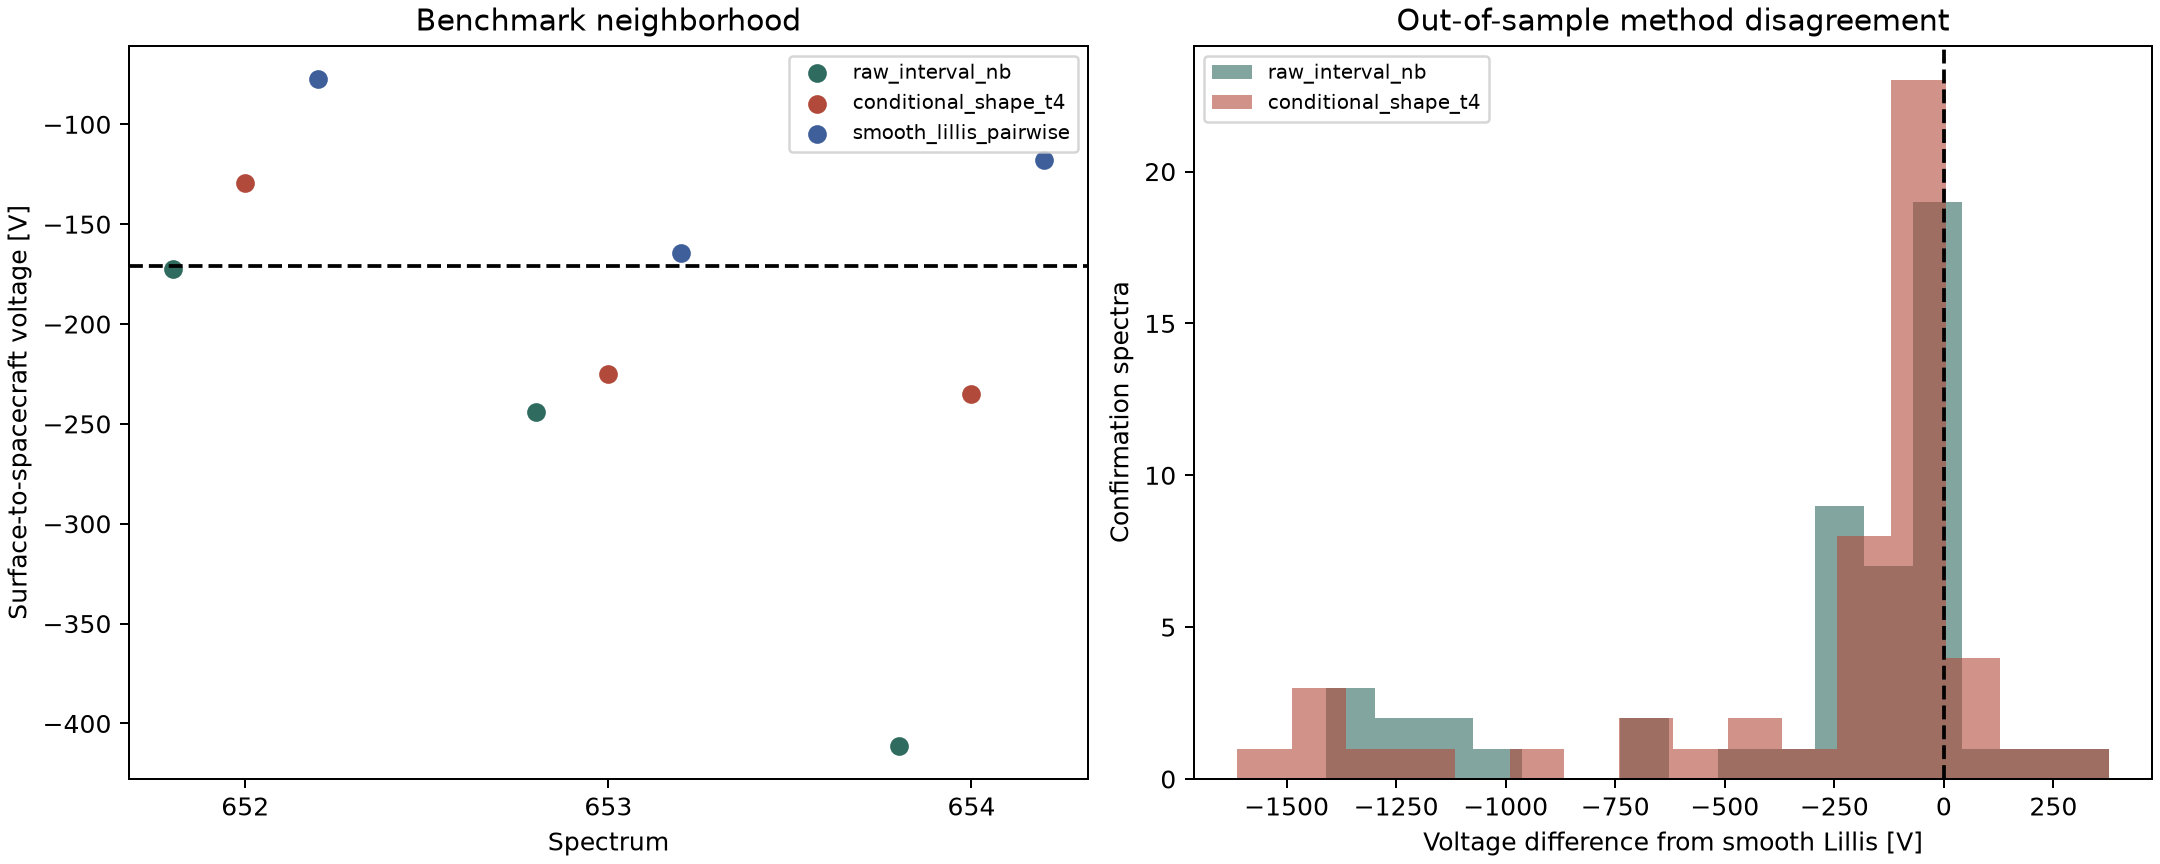
\includegraphics[width=0.95\linewidth]{../comparison.png}
  \caption{Benchmark estimates (left) and out-of-sample voltage differences
  from smooth Lillis (right).}
  \label{fig:comparison}
\end{figure}

\section{Matched-Simulation Analysis}

To distinguish estimator failure from model misspecification, each objective is
tested under its own assumed observation model.  We set
$\UM=-160$~V, $\BSBM=0.975$, and $A_b=0.621$, hold nuisance parameters fixed,
and evaluate a two-volt voltage profile.  Thirty simulations calibrate profile
thresholds and sixty independent simulations evaluate coverage.  This is a
conditional voltage test, not full three-parameter coverage.

\begin{table}[ht]
\centering
\caption{Matched-simulation performance.  Coverage uses empirically calibrated
profile thresholds; median error refers to the point estimate.}
\label{tab:coverage}
\begin{tabular}{lrrr}
\toprule
Method & Median $|\widehat U-U|$ (V) & 68\% coverage & 95\% coverage \\
\midrule
Raw interval negative binomial & 4 & 0.62 & 0.83 \\
Conditional log shape & 6 & 0.58 & 0.90 \\
Smooth pairwise Lillis & 9 & 0.72 & 0.93 \\
\bottomrule
\end{tabular}
\end{table}

The small calibration set makes the empirical upper quantiles noisy.  The
nominal likelihood thresholds give 95\% coverage of 0.95 for interval counts
and 0.93 for conditional shape.  Therefore the count and conditional estimators
are capable of recovering voltage under matched assumptions.  Their real-data
failure cannot be attributed simply to a broken optimizer or absence of voltage
information in the mathematical objective.

\section{Interpretation of the Three Attempts}

\subsection{Why corrected counts did not solve the benchmark}

The 120.9-fold count correction removes false precision but does not change
which residual patterns receive relatively high count weight.  Broad reflected
enhancements, energy-dependent angular response, or an incorrect incident
distribution can still pull $\UM$ because the count likelihood interprets them
through the available loss-cone, magnetic-ratio, and beam parameters.  The
negative-binomial term widens variance; it does not remove systematic residual
direction.  The count fit's $-244$~V benchmark and beam-bound solution show
that remaining discrepancy is not exchangeable noise alone.

\subsection{Why conditional shape was not enough}

Centering log flux removes row intensity and reduces dependence on absolute
response, but it preserves angular residual structure.  A robust Student-$t$
loss limits isolated outliers; it cannot distinguish a coherent unmodeled beam
or response pattern from a shifted loss-cone boundary.  The intermediate
$-225$~V result is consistent with partial robustness, not complete removal of
the confounding structure.

\subsection{Why Lillis can be right for the wrong reasons}

Pairwise normalization strongly suppresses incident-side intensity and gives
equal linear-residual influence rather than count influence.  On the published
example this recovers both voltage and magnetic ratio.  However, the beam bound
and confirmation instability prevent interpreting benchmark agreement as
proof that the complete physical model is correct.  Lillis is presently the
best benchmark-preserving diagnostic, but not a validated production
likelihood.

\section{Decision and Consequences}

No candidate satisfies all frozen gates.  Raw interval counts and conditional
shape fail the positive benchmark and confirmation-stability criteria.  Smooth
Lillis passes the benchmark but fails nuisance-bound and broad confirmation
criteria.  Consequently:
\begin{enumerate}
  \item no observation model is promoted to production;
  \item count reconstruction should remain corrected and interval-aware in
  future experiments, because the old count scale is demonstrably wrong;
  \item the next work should revise or test the forward model before assigning
  final uncertainty;
  \item candidate refinements should examine beam functional form and bounds,
  incident-distribution anisotropy, energy-dependent angular response,
  spacecraft-potential uncertainty, and plasma-regime screening;
  \item confirmation spectra with boundary solutions should be treated as
  non-identifiable rather than reported as extreme physical potentials.
\end{enumerate}

\section{Limitations}

The effective response is locally calibrated from paired Level-0 and Level-1
data and is not yet established mission-wide.  Spacecraft potential is fixed at
+11~V for comparability with the published benchmark.  A single discovery
overdispersion and conditional scale are used across changing plasma regimes.
The matched-simulation coverage study fixes magnetic ratio, beam amplitude, and
mask, so it is intentionally less demanding than full retrieval coverage.
Finally, this experiment compares observation models while holding the forward
physics constant; it cannot identify which missing physical component causes
the residual structure.

\section{Reproducibility}

The frozen panel is in \code{panel\_manifest.csv}.  Real-data fits are in
\code{results.csv}; seed checks are in \code{seed\_stability.csv}; matched
simulation results are in \code{coverage.csv}; and telemetry provenance is in
the Experiment-002 source ledger.  The implementation is entirely under
\code{experiments/experiment-003/} and does not alter production source.

\begin{thebibliography}{9}
\bibitem{halekas2008}
J. S. Halekas et al., ``Lunar Prospector observations of the electrostatic
potential of the lunar surface and its response to incident currents,''
\emph{Journal of Geophysical Research}, 2008,
doi:10.1029/2008JA013194.

\bibitem{magerfmt}
Lunar Prospector Project, \emph{LP MAG/ER Telemetry Format}, governing Format-3
archive document,
\url{https://pds.nasa.gov/data/lp-l-6-position-v1.0/lp_0016/document/magerfmt.pdf}.

\bibitem{pds3d}
NASA Planetary Data System, \emph{Lunar Prospector Electron Reflectometer
3-D Electron Flux Data Set Description},
\url{https://pds-ppi.igpp.ucla.edu/archive1/LP_1204/CATALOG/ER3D_DS.CAT}.
\end{thebibliography}

\end{document}
